\documentclass{beamer}
\usepackage{color}
\usepackage{hyperref}
% \usepackage{pgf, pgfarrows, pgfnodes}
\usepackage{mathtools}
\usetheme{AnnArbor}
\title[https://github.com/cheraaqee/popSR]{Perceptually-Optimized Loss Function for Image Super-Resolution}
\author[ICSPIS2021]{\small Amirhossein Arezoomand \inst{1} \and Pooryaa Cheraaqee \inst{1} \and Azadeh Mansouri \inst{1}}
\institute[]{\inst{1} \textbf{Department of\\ Electrical and Computer Engineering,\\ Kharazmi University}}
% \date{\today}
\begin{document}
%%%%
\begin{frame}
\frametitle{ICSPIS 2021}
\titlepage
\end{frame}
%%%%
\section*{Outline}
\begin{frame}
\frametitle{Outline}
\tableofcontents[pausesections]
\end{frame}
%%%
\section{Problem Definition}
\subsection{Image Super-Resolution}
\begin{frame}
\frametitle{What is \emph{Super-Resolution}?}
\begin{itemize}
\visible<1->{
\item increasing the dimension}
\begin{itemize}
\visible<2,3>{
\item $\text{input (}X_{M\times N}) \xrightarrow{\text{upsampling by a factor of 2 (i.e. }2\uparrow)} \text{output (}Y_{2M\times 2N})$}
\visible<3>{
\item BiLinear, BiCubic, etc.}
\end{itemize}
\visible<4->{
\item
\textcolor{red}{\textbf{!! Preserving the quality !!}}}
\end{itemize}
\visible<5->{
\begin{center}
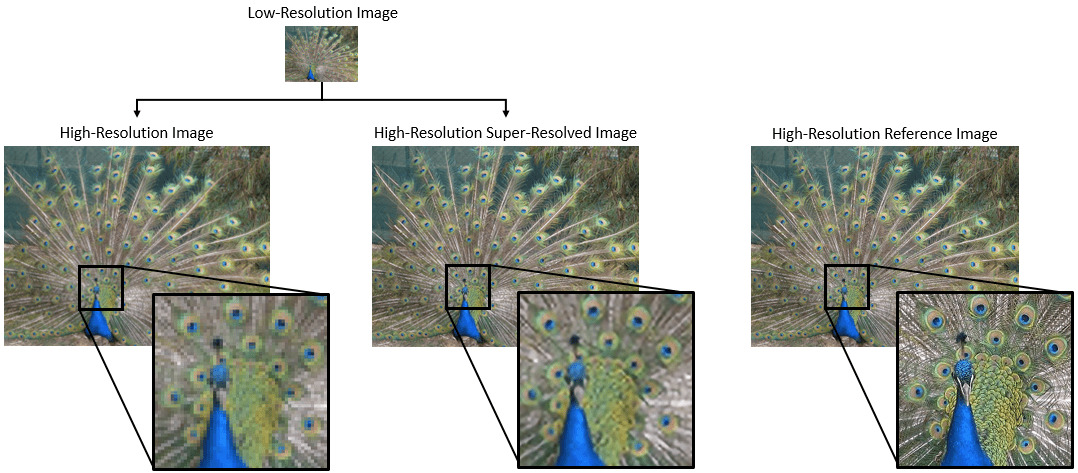
\includegraphics[height=4cm]{sr_sample}
\end{center}
}
\end{frame}
\subsection{Loss Function}
\begin{frame}
\frametitle{CNNs and Loss Functions}
\begin{itemize}
\visible<1->{
\item Super-Resolver CNNs
\vskip 0.5cm
	\only<2-5>{
		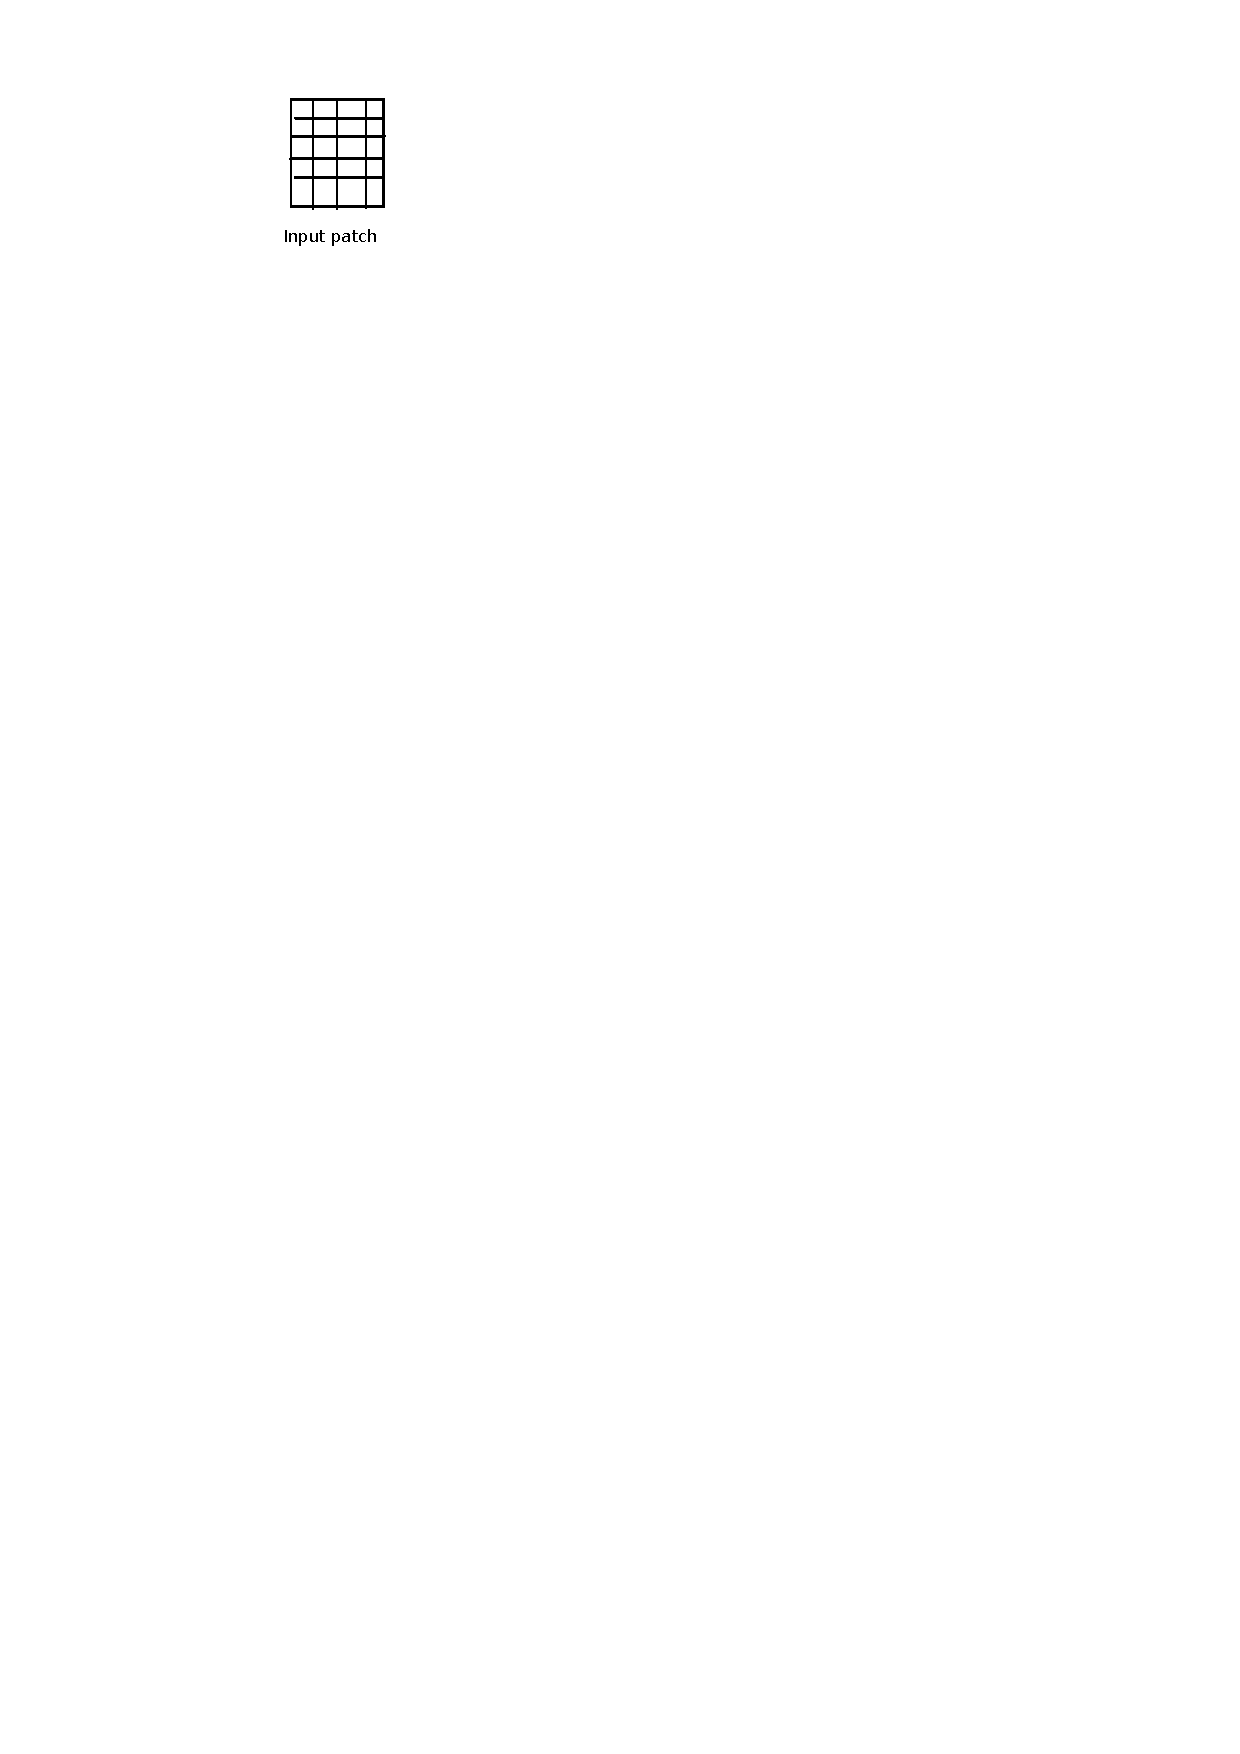
\includegraphics[trim={4.7cm, 25.5cm, 14.5cm, 2cm}, clip, width=1cm]{figure_slide}}
	\only<3-5>{
		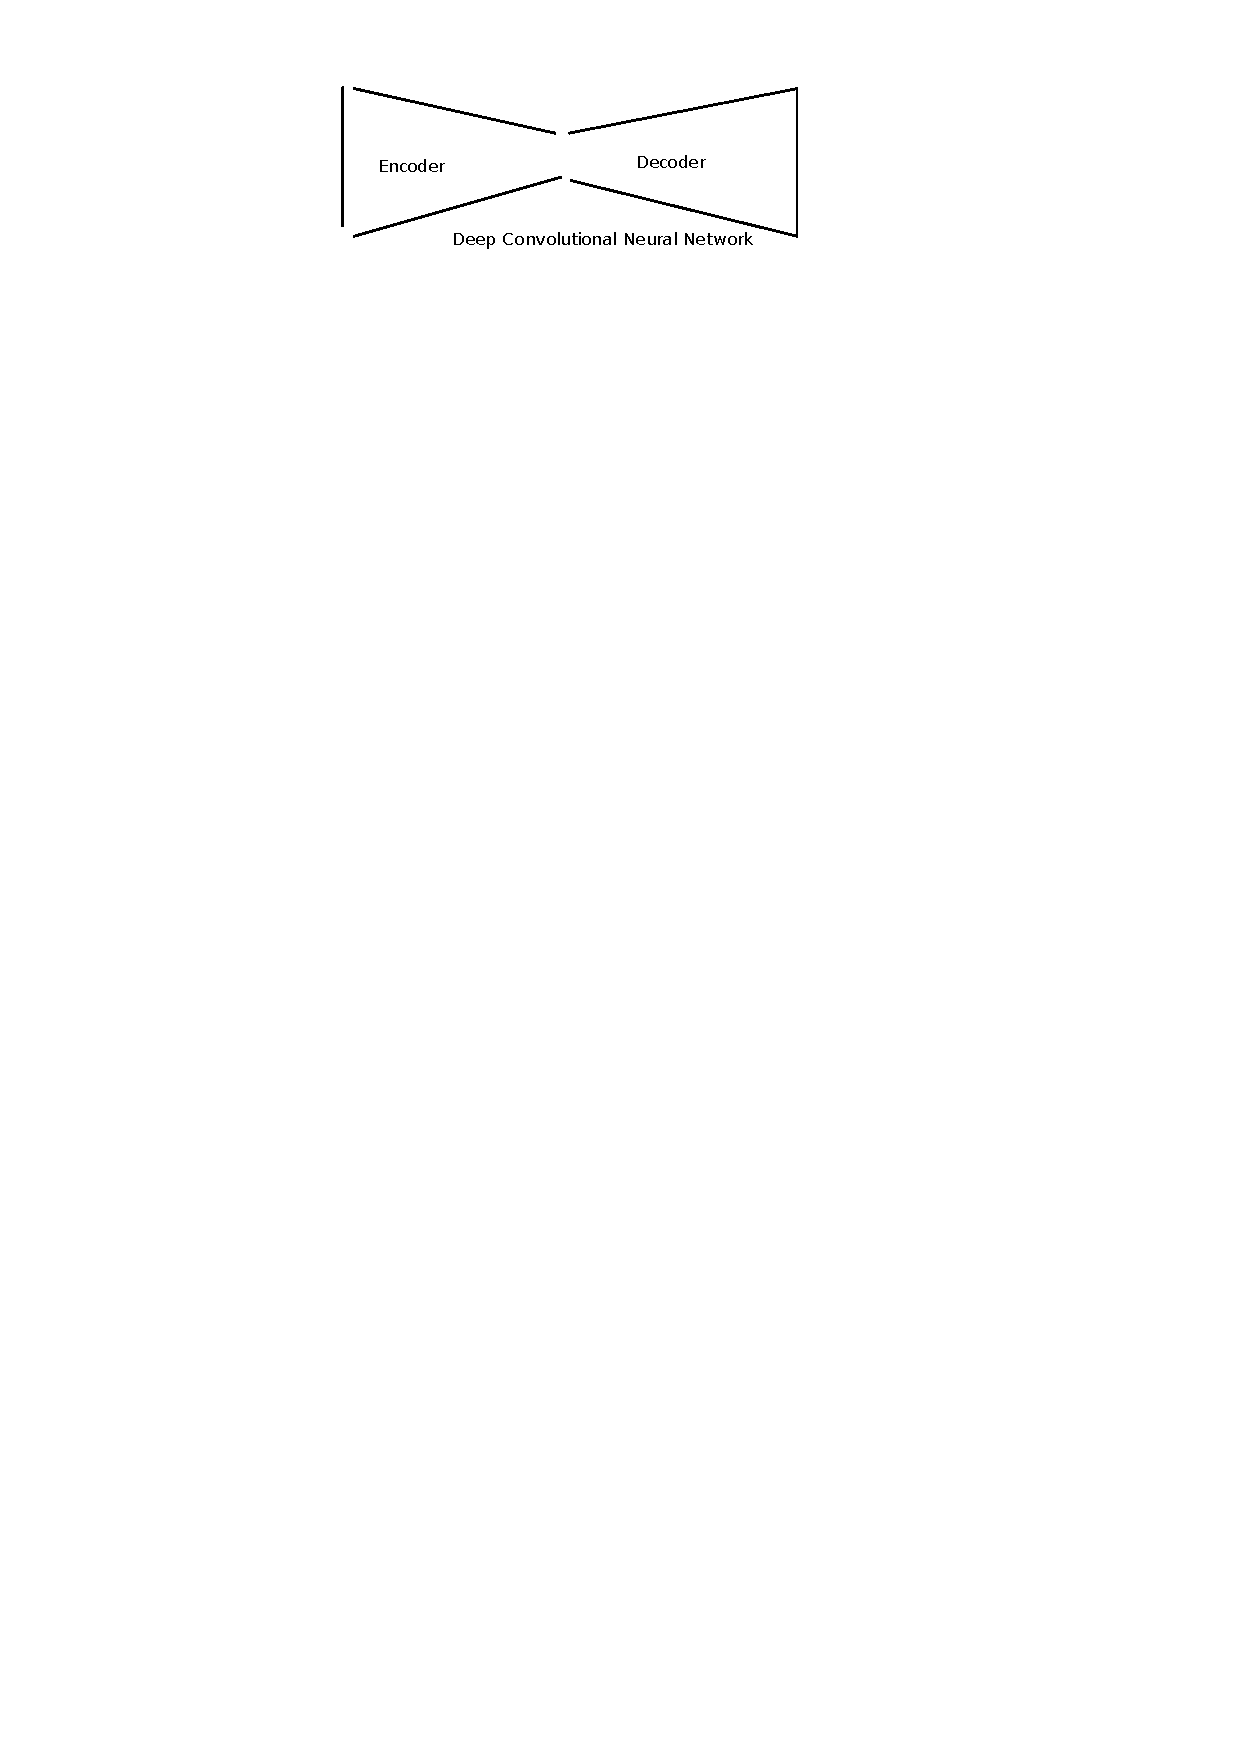
\includegraphics[trim={5.7cm, 25.5cm, 7.3cm, 1.3cm}, clip,width=5cm]{figure_Cnn}}
	\only<4-5>{
		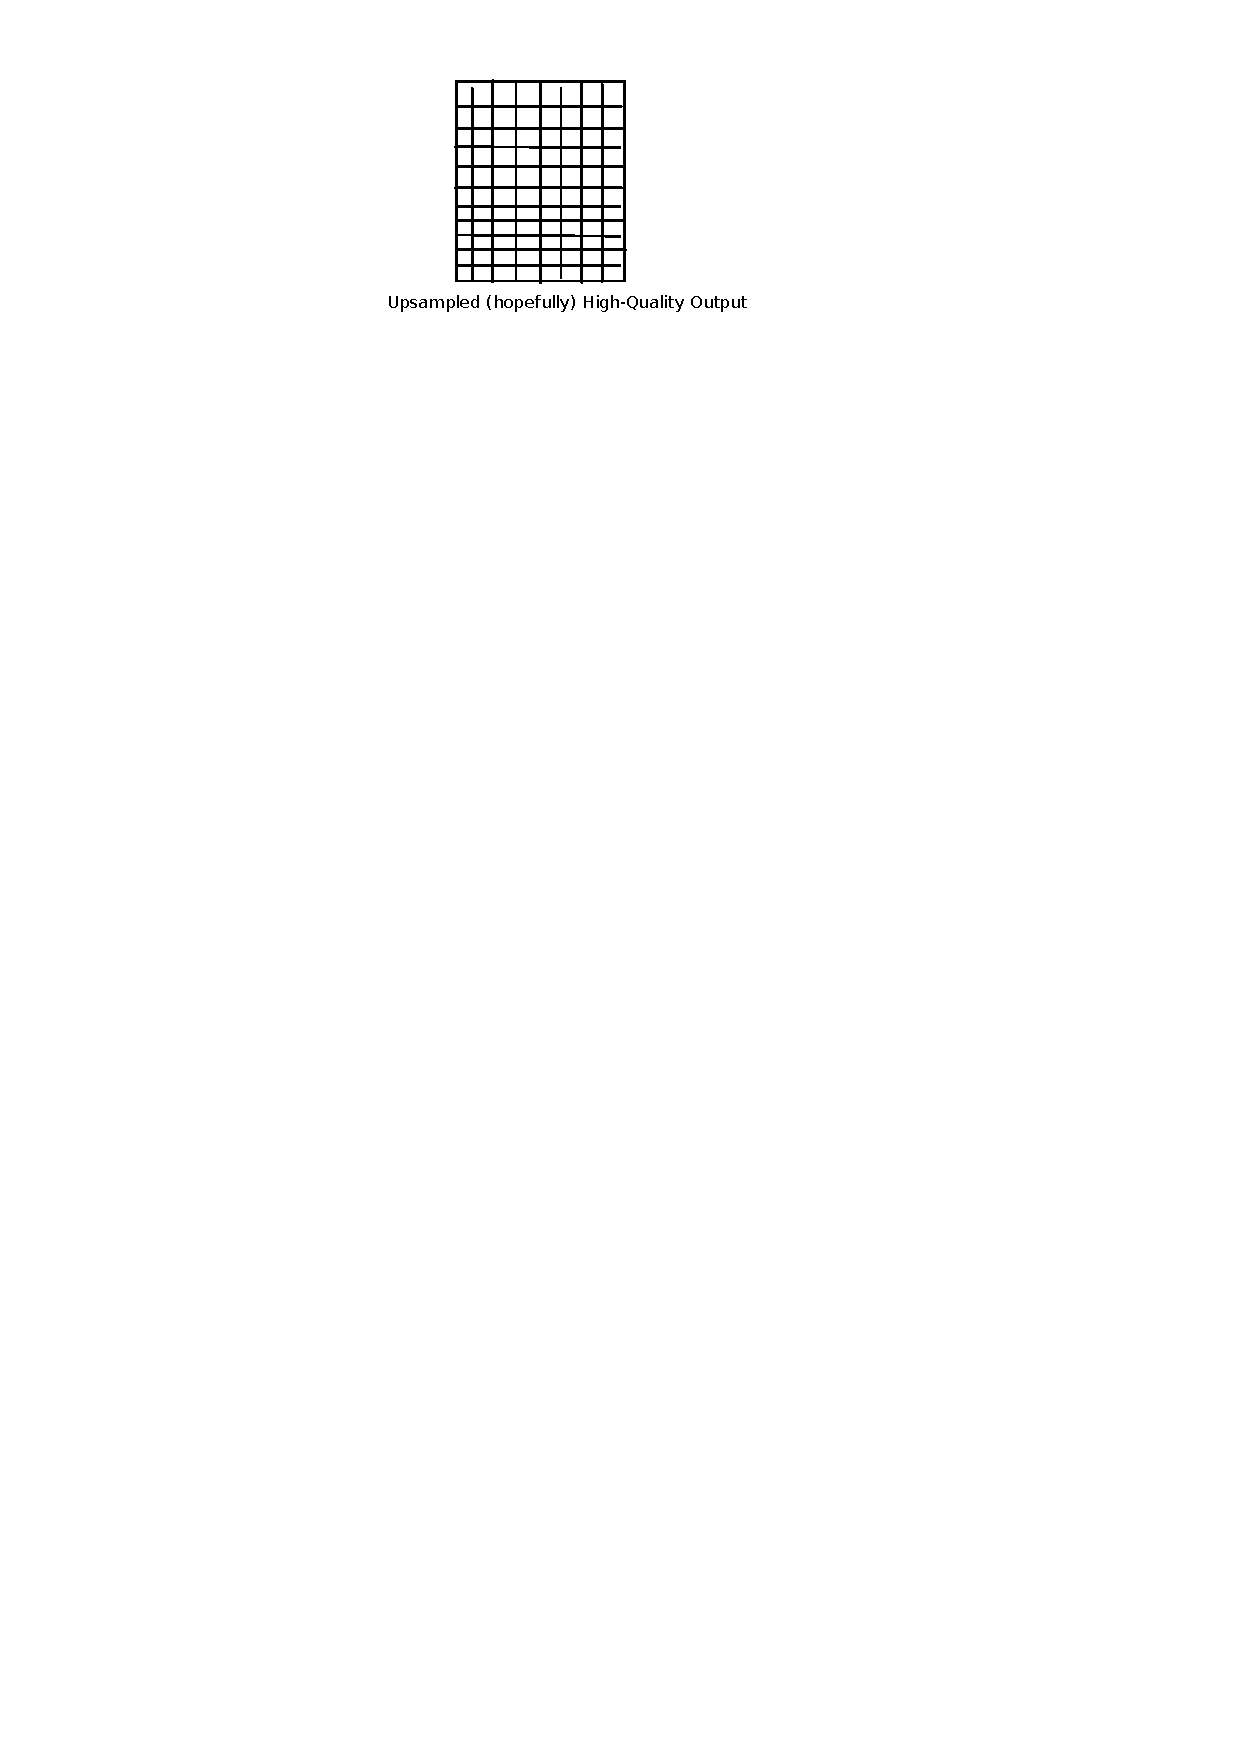
\includegraphics[trim={6.55cm, 24.3cm, 8.2cm, 1.2cm}, clip, width=3cm]{figure_output}}

	\only<5>{
		\hskip 6.5cm 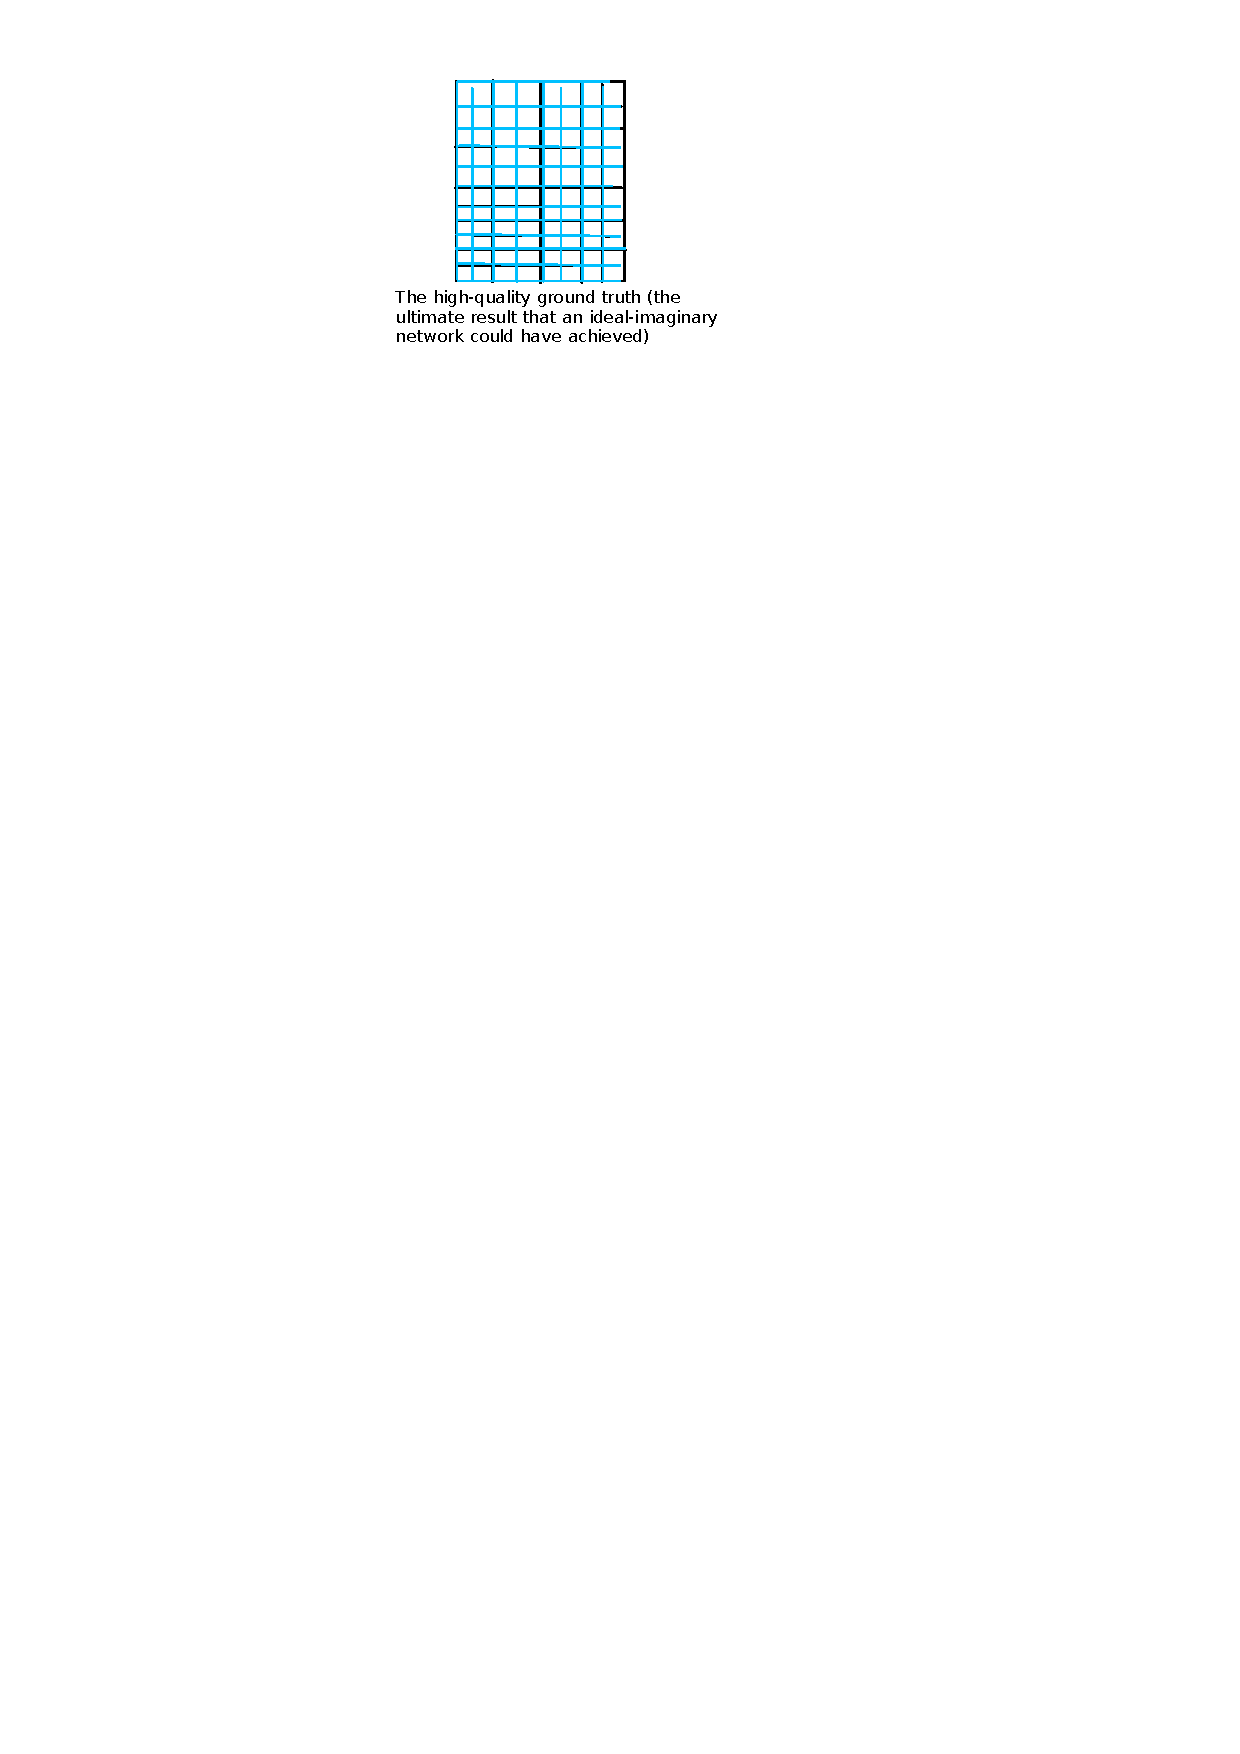
\includegraphics[trim={6.55cm, 23.3cm, 8.5cm, 1.2cm}, clip, width=3cm]{figure_gt}}
}
% \visible<6->{
% 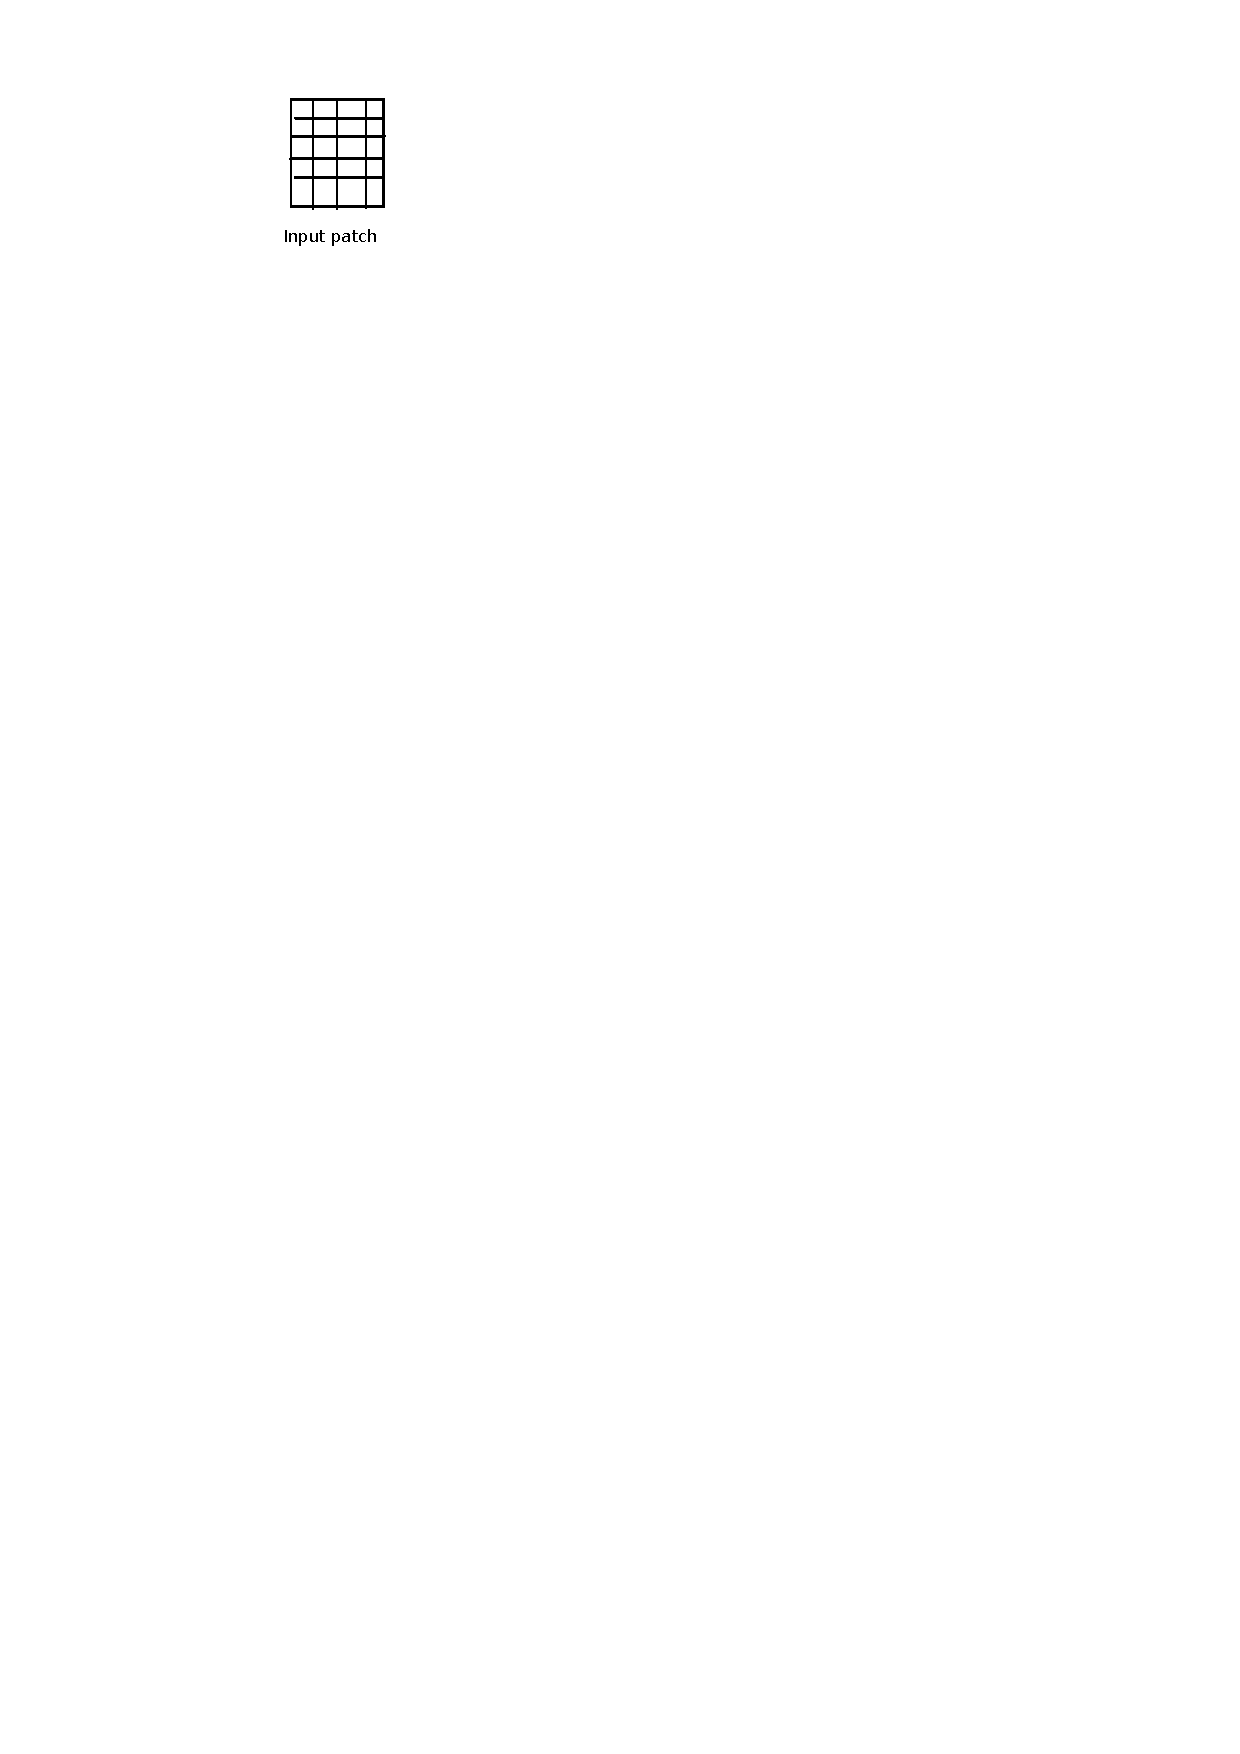
\includegraphics[trim={4.7cm, 25.5cm, 14.5cm, 2cm}, clip, width=1cm]{figure_slide}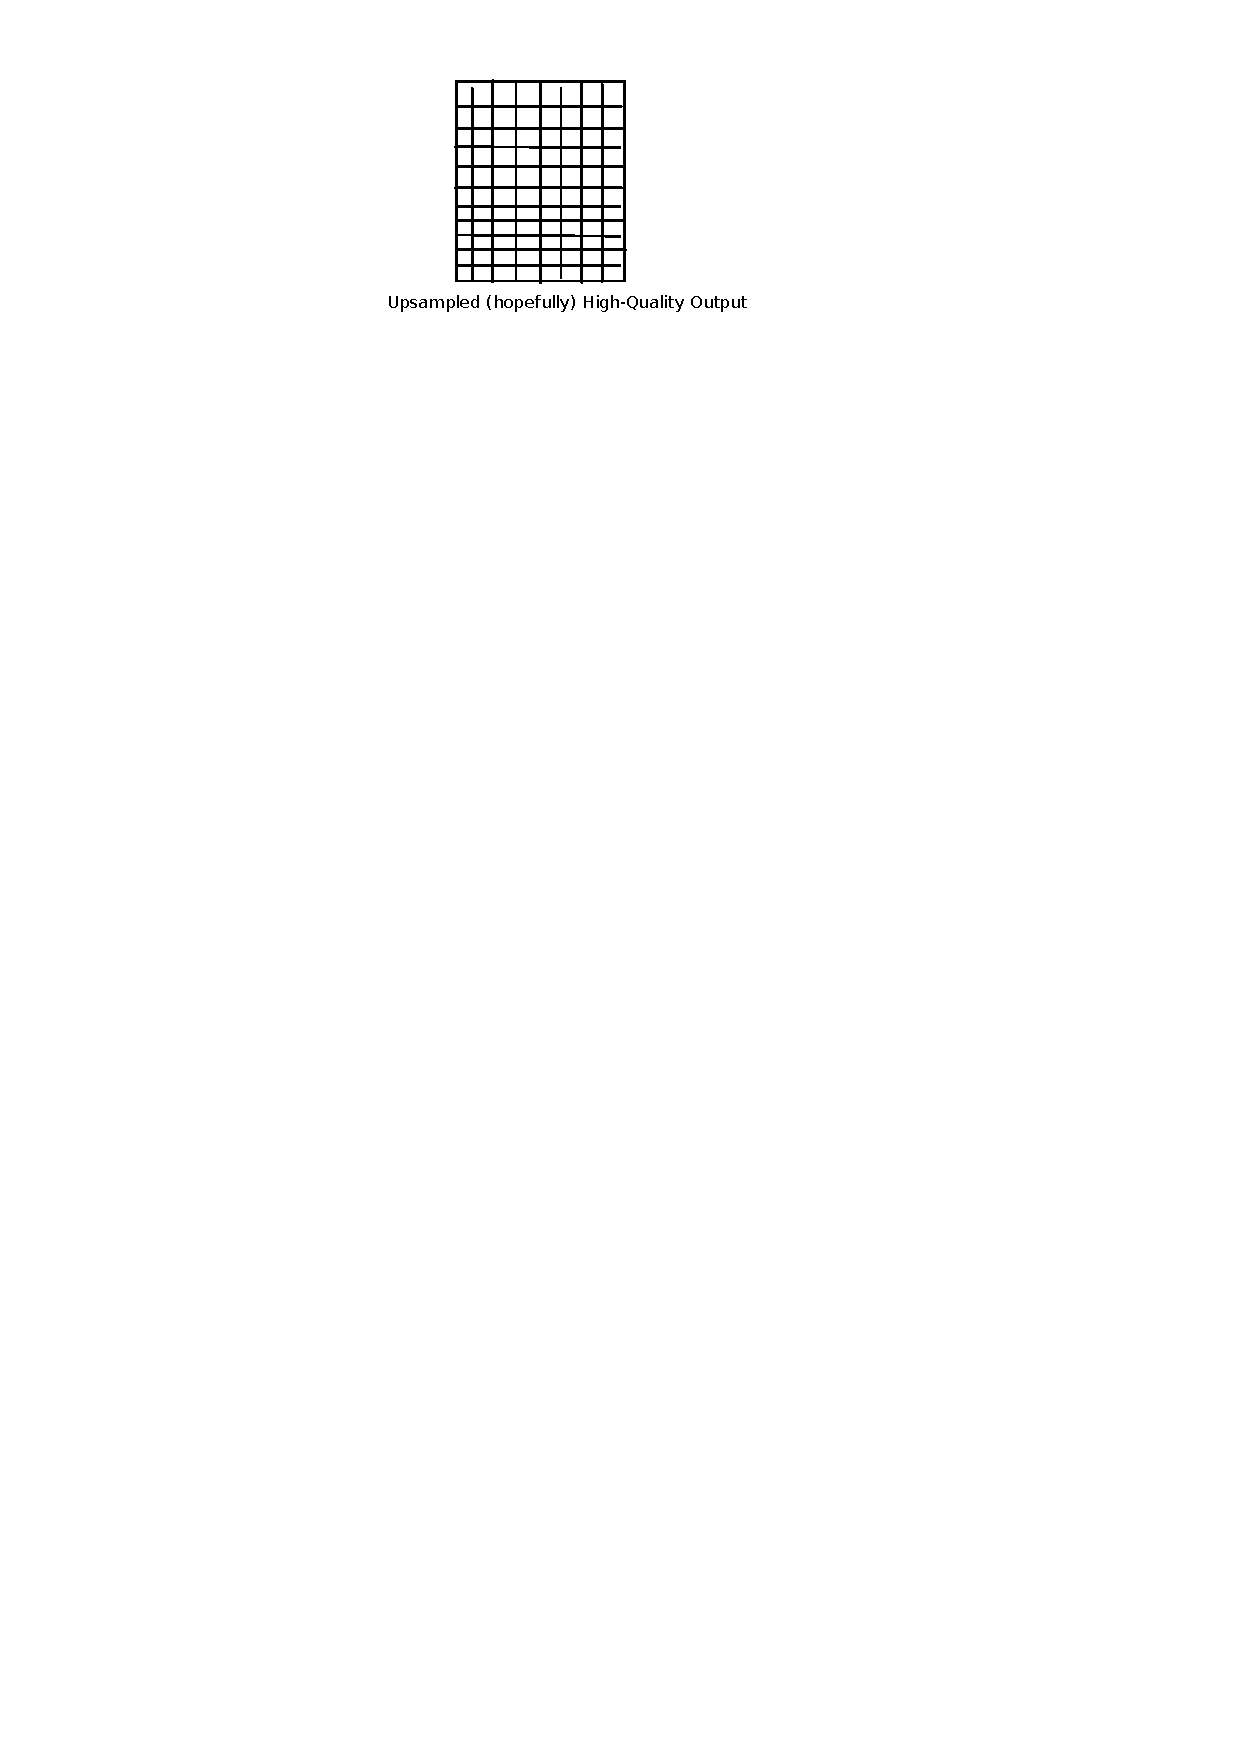
\includegraphics[trim={6.55cm, 24.3cm, 8.2cm, 1.2cm}, clip, width=3cm]{figure_output}
% 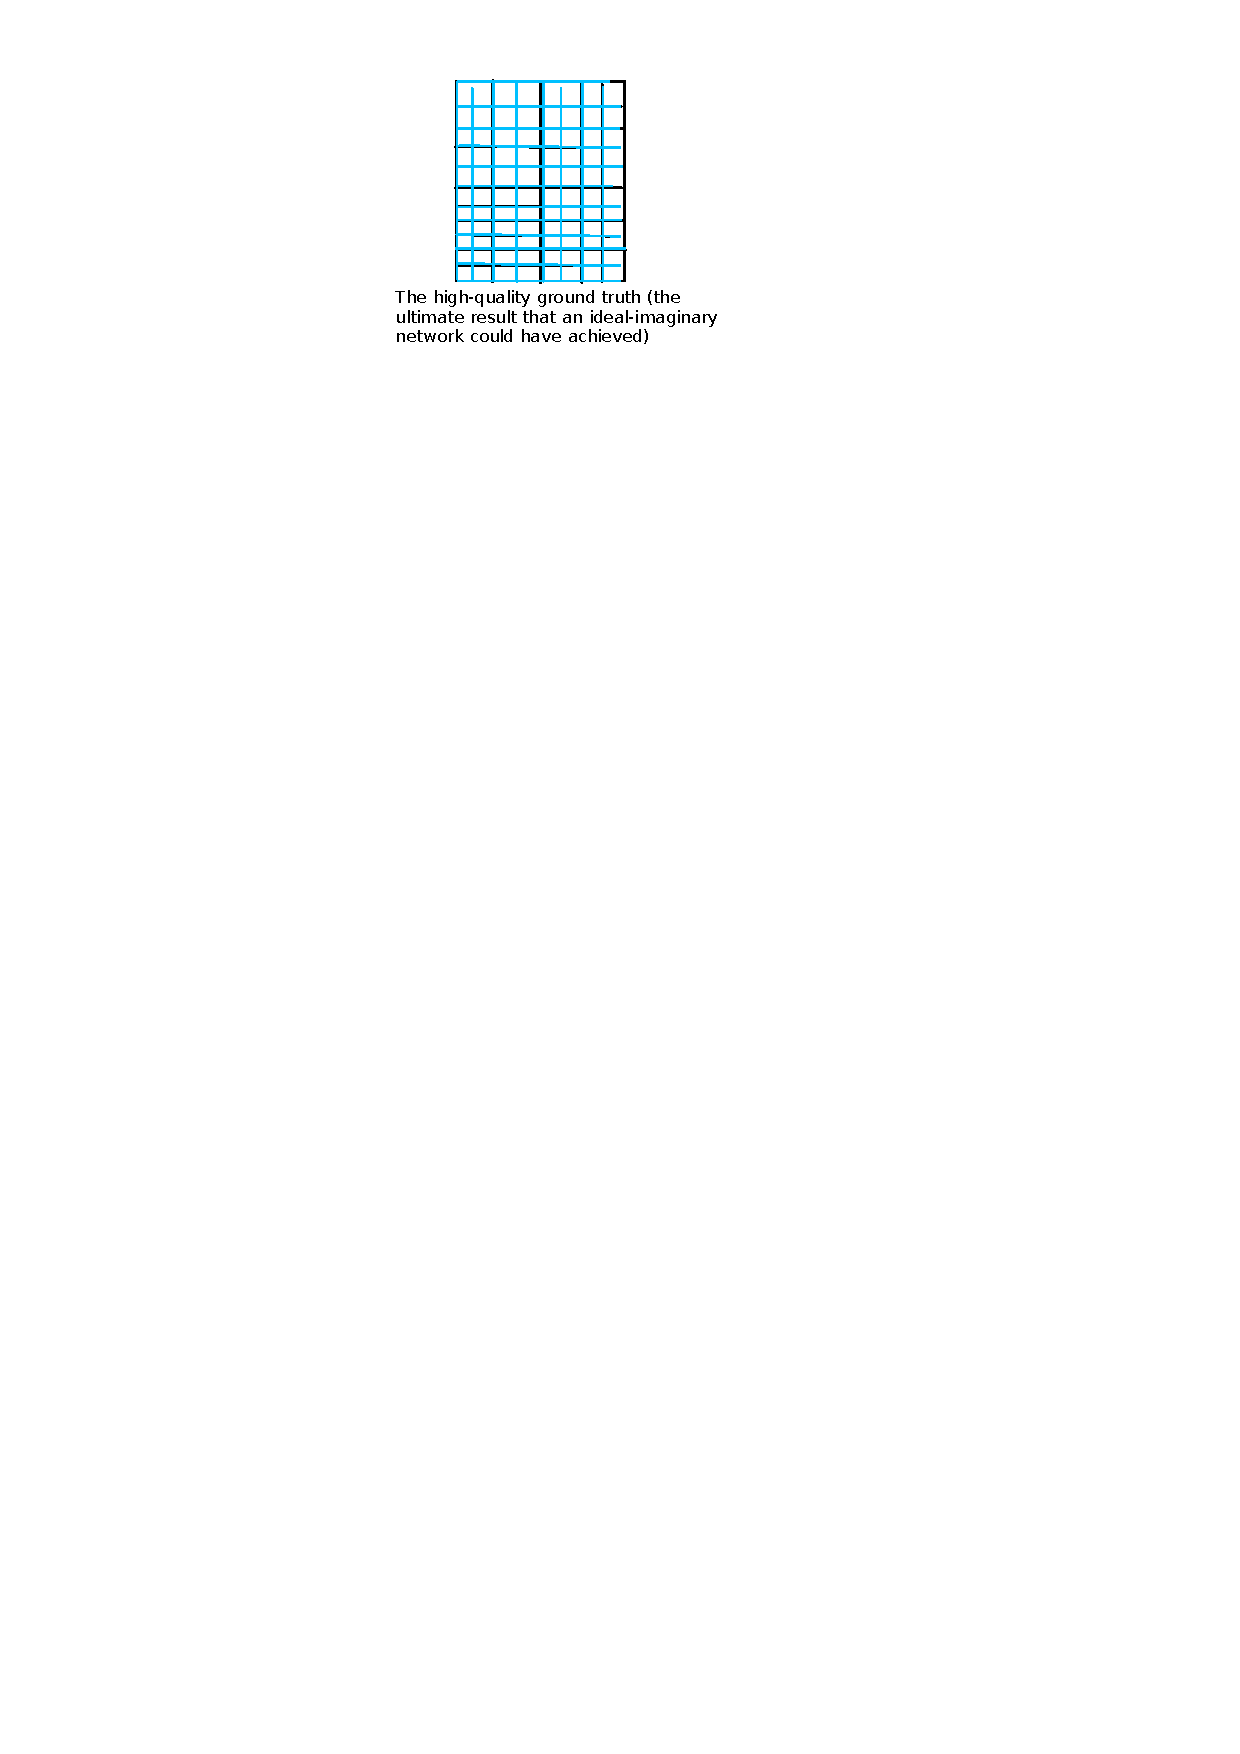
\includegraphics[trim={6.55cm, 23.3cm, 8.5cm, 1.2cm}, clip, width=3cm]{figure_gt}
% }
\visible<7->{
\item The Loss Function
	
	\only<8-14>{$X\rightarrow \text{Network's input}$}

		\only<9-14>{$\hat{Y}\rightarrow \text{Network's output}$}

		\only<10-14>{$Y\rightarrow \text{The correct answer}$}

		\only<11-14>{$W\rightarrow \text{Current network's weight}$}

		\only<12-14>{$Y=F(X, W)$}

		\only<13-14>{\small{The amount of update that must be applied to} $W~(i.e. \Delta W) = E(Y, \hat{Y})$; where $E\in[0,1]$}

		\only<14>{\small{The updated network's weights} $(i.e. W\prime) = W+\Delta W$}

		\onslide<15>{\textbf{How to define $E(Y, \hat{Y})$}?}
}
\end{itemize}
\end{frame}
%%%
\section{Previous Attempts}
\begin{frame}
	\frametitle{Ways to Define a Loss Function}
	\begin{itemize}
	\visible<2->{\item Visible Error}

		\visible<3->{
			$\displaystyle E(Y, \hat{Y})=\frac{1}{M\times N}\sum_{i=1}^M{\sum_{j=1}^N{(Y(i, j)-\hat{Y}(i, j))^2}}$
			}
		\visible<4->{\item Quality Metrics}
		
		\visible<5->{
			$E(Y, \hat{Y})=SSIM(Y, \hat{Y})$
			}

		\visible<6->{
			\begin{center}
				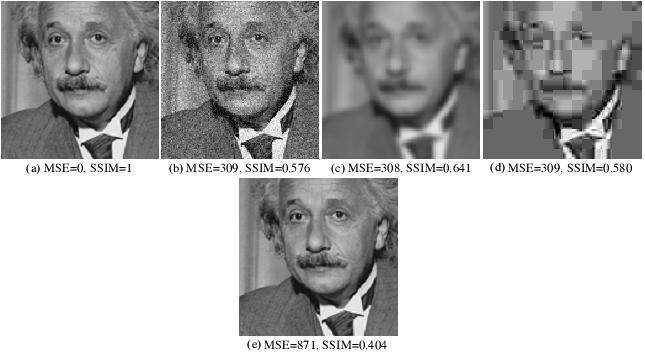
\includegraphics[width=8cm]{ssim_vs_mse}
			\end{center}
			}
	\end{itemize}
\end{frame}
%%%
\section{The Taken Approach}
\begin{frame}
\frametitle{Our Approach}
\begin{itemize}
\visible<2->{
\item DCT
\begin{itemize}	
\visible<3->{
\item Expressive
\only<4-5>{

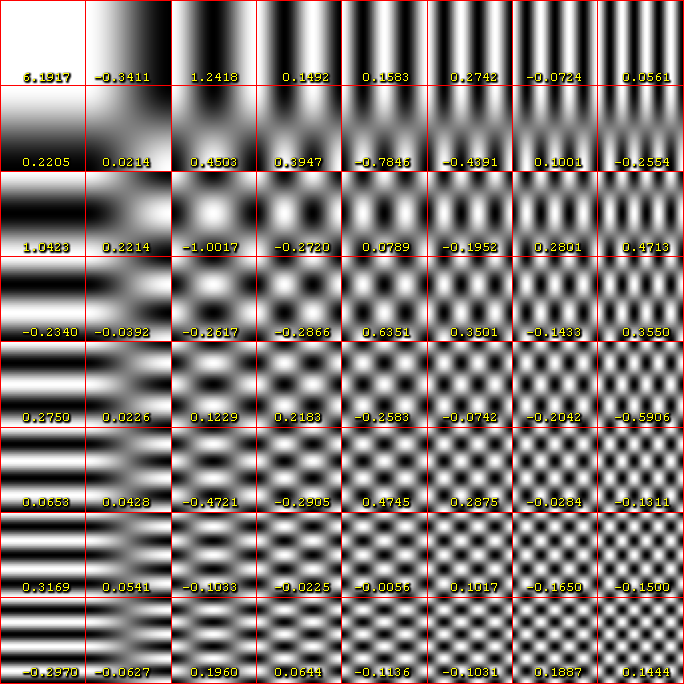
\includegraphics[width=3cm]{figure_dct_kernels}
}
\only<5>{
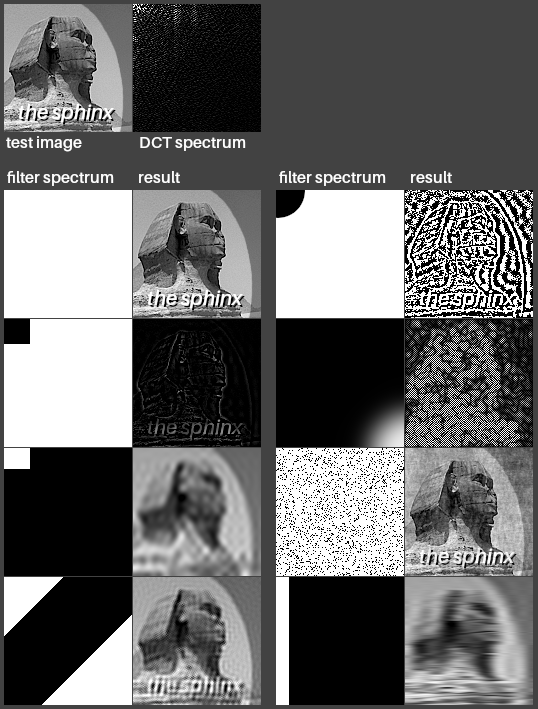
\includegraphics[width=5cm]{figure_dct_examples}
}
}
\visible<6->{
\item Fast!
}
\end{itemize}
}
\visible<7->{
\item Further Purification
	
}
\end{itemize}

\end{frame}
%%%
\section{Results}
\subsection{Quantitative}
\subsection{Qualitative}
%%%%
\section{Conclusion\& Future Works}
\end{document}
